\section{Graph Programs}
\label{sec:graph-programs}

This paper focusses on GP~2, a successor to the graph programming language GP \cite{Plump09a,Plump12a}.
GP is a domain-specific language which aims to support formal reasoning on graph programs (see \cite{Poskitt-Plump12a} for a Hoare-logic approach to verifying GP programs). We give a brief introduction to GP~2, mainly by example. The definition of the language, including a formal operational semantics, can be found in \cite{Plump12a}. 

A graph program consists of declarations of conditional graph transformation rules and macros, and exactly one main command sequence. Graphs are directed and may contain  loops and parallel edges. The rules operate on a \emph{host graph}\/ (or input graph) whose nodes and edges may be labelled.

Labels are of type \texttt{int} (for integers), \texttt{char} (for characters), \texttt{string} (for character strings), \texttt{atom} or \texttt{list}, where \texttt{atom} is the union of \texttt{int}, \texttt{char} and \texttt{string}. Atoms are considered as lists of length one, hence integers and strings are also lists. Given lists $\mtt{x}$ and $\mtt{y}$, their concatenation is written \texttt{x:y} (not to be confused with the list-cons operator in Haskell). 
We proceed by discussing two example programs.

\begin{example}[Transitive Closure]
The principal programming constructs in GP~2 are conditional graph-transformation rules labelled with expressions. The program in Figure \ref{fig:transitive-closure} applies the single rule \ttt{link} \emph{as long possible} to a host graph. In general, any subprogram can be iterated by applying \ttt{!} as a postfix operator.

\begin{figure}[htb]
\begin{center}
 \input{Programs/trans_closure.prog}
\end{center}
%\vspace{-.5\baselineskip}
\caption{Program for transitive closure}\label{fig:transitive-closure}
\end{figure}

Applying \ttt{link} amounts to non-deterministically selecting a subgraph of the host graph that matches \ttt{link}'s left graph, and adding to it an edge from node 1 to node 3 provided there is no such edge (with any label). The application condition ensures that the program terminates and extends the host graph with a minimal number of edges.

A graph is \emph{transitive} if for each directed path from a node $v$ to another node $v'$, there is an edge from $v$ to $v'$.  Given any graph $G$, the program in Figure \ref{fig:transitive-closure} produces the smallest transitive graph that results from adding unlabelled edges to $G$.\footnote{``Unlabelled'' edges are actually labelled with the empty list.} This graph is unique up to isomorphism and requires at most $n^2$ applications of \ttt{link}, where $n$\/ is the number of nodes in $G$. \qed
\end{example}
  

\begin{example}[Vertex Colouring]
The program in Figure \ref{fig:vertex-colouring} assigns a \emph{colour}\/ to each node of the host graph, such that non-loop edges have differently coloured endpoints. Positive integers are used as colours because, in general, an unbounded number of colours is needed. The program replaces each node label $l$\/ with $l{:}i$, where $i$\/ is the node's colour. In addition, the rule \ttt{init} shades nodes to prevent repeated application to the same node.
% (Nodes can be graphically \emph{marked}\/ by drawing them shaded or in one of the colours red, green or blue.)

\begin{figure}[htb]
\begin{center}
 \input{Programs/vertex-colouring.prog}
\end{center}
%\vspace{-.5\baselineskip}
\caption{Program for vertex colouring}\label{fig:vertex-colouring}
\end{figure}

Rule \ttt{inc} is applied to the host graph as long as there are edges with identically coloured endpoints. It can can be shown that this terminates after at most $n^2$ rule applications, where $n$\/ is the number of nodes. In contrast to the previous example program, \emph{different graphs may result}\/ from this process. In particular, there is no guarantee that the number of colours produced is minimal. For instance, Figure \ref{fig:colour_results} shows two different colourings produced for the same host graph.
\qed
\end{example}

\begin{figure}[htb]
\begin{center}
 \input{Graphs/colour_results.graph}
\end{center}
%\vspace{-.5\baselineskip}
\caption{Different results from vertex colouring}\label{fig:colour_results}
\end{figure}

\vspace{.5\baselineskip}
\noindent
\emph{Other program constructs.}
A GP~2 command not used in the example programs is a rule set $\mtt{\{}r_1,\dots,r_n\mtt{\}}$. This command \emph{non-deterministically} applies any of the rules to the current host graph. The application \emph{fails}\/ if none of the left-hand graphs in the rules matches a subgraph. Matches must be injective and are only valid if they do not result in \emph{dangling edges}.

Another construct not yet discussed is the branching command \ttt{if} $C$ \ttt{then} $P$ \ttt{else} $Q$, where $C$, $P$ and $Q$ are arbitrary command sequences. This is executed on a host graph $G$ by first executing $C$ on a copy of $G$. If $C$ succeeds, $P$\/ is executed on the original graph $G$; otherwise, $Q$ is executed on $G$. The command \ttt{try} $C$ \ttt{then} $P$ \ttt{else} $Q$ has a similar effect, except that $P$\/ is executed on the graph resulting from $C$'s execution. 

\section{Benchmark Programs}
\label{sec:benchmark}
 
Besides the programs for transitive closure and vertex colouring, we select four more programs for benchmarking.


\subsection{Shortest distances}

\begin{tabular}{lp{10.5cm}}
\ul{Input:} & A graph $G$ with a unique grey node $s$. All edge labels are non-negative integers. \\
\ul{Output:} & The graph obtained from $G$ by marking grey each node reachable from $s$ and replacing its label $l$\/ with $l{:}d$, where $d$\/ is the shortest distance from $s$. (A distance is the sum of the edge labels of a directed path.)
\end{tabular}
  
\begin{center}
\input{Programs/distances.prog}
\end{center}

\ul{Notes}
\begin{enumerate}
\setlength{\itemsep}{-.5ex}
\item The output is unique up to isomorphism.
\item The input requirement can be relaxed by allowing negative edge labels but forbidding directed cycles with a negative distance.
\end{enumerate}


\subsection{Recognising acyclic graphs}
\label{sec:acyclic}

\begin{tabular}{lp{10.5cm}}
\ul{Input:} & Any graph $G$. \\
\ul{Output:} & Graph $G$ if it is acyclic, otherwise the program fails.
\end{tabular}
  
\begin{center}
\input{Programs/acyclic.prog}
\end{center}


\subsection{Rooted 2-colouring}

\begin{tabular}{lp{10.5cm}}
\ul{Input:} & A non-empty, single-rooted, connected graph $G$ with atomic labels. \\
\ul{Output:} & If $G$\/ is 2-colourable, then the output is obtained from $G$\/ by marking each node with either red or blue. The source and target of each non-loop edge have different colours.\\
& If $G$\/ is not 2-colourable, then the output is $G$.
\end{tabular}

\begin{center}
\begin{tikzpicture} [scale=0.7,align=center,auto,inner sep=2mm,arrowin,arrowout,font=\ttfamily]
\node at (4.75,3.8) {main = try (init; colouring; unshaded)};
\node at (6.75,3.2) {colouring = ((colour; if invalid then stop)!; back)!};
\node at (4,2.6) {colour = \{colour-blue,colour-red\}};
\node at (4.45,2) {invalid = \{joined-reds,joined-blues\}};

%init
\node at (0,0)[root,label=below:\scriptsize{1}]{x};
\node at (1.2,0){$\Rightarrow$};
\node at (1,0)[above=5mm] {init(x:atom)};
\node at (2.4,0)[root,fill=red!75,label=below:\scriptsize{1}]{x};

%stop
\begin{scope}[yshift=-3cm]
\node (l1) at (0,0)[root,label=below:\scriptsize{1}]{x};
\node at (1.2,0){$\Rightarrow$};
\node at (1,0)[above=5mm] {stop(x:atom)};
\node (r1) at (2.4,0)[root,fill=black!20,label=below:\scriptsize{1}]{x};
\end{scope}

%unshaded
\begin{scope}[yshift=-6cm]
\node (l1) at (0,0)[root,label=below:\scriptsize{1}]{x};
\node at (1.2,0){$\Rightarrow$};
\node at (1.5,0)[above=5mm] {unshaded(x:atom)};
\node (r1) at (2.4,0)[root,label=below:\scriptsize{1}]{x};
\end{scope}

%colour-red
\begin{scope}[xshift=5.5cm]
\node (l1) at (0,0)[root,fill=red!75,label=below:\scriptsize{1}]{x};
\node (l2) at (2.9,0)[inner sep = 2mm,circle,draw,label=below:\scriptsize{2}]{y}
   edge [-] node[above]{a} (l1);
\node at (4.1,0){$\Rightarrow$};
\node at (3.2,0)[above=5mm] {colour-red(a:list; x,y:atom)};
\node (r1) at (5.3,0)[circle,draw,fill=red!75,label=below:\scriptsize{1}]{x};
\node (r2) at (8.2,0)[root,fill=blue!60,label=below:\scriptsize{2}]{y}
  edge [-,dashed] node[above]{a} (r1);  
\end{scope}

%joined-reds
\begin{scope}[xshift=5.5cm,yshift=-3cm]
\node (l1) at (0,0)[root,fill=red!75,label=below:\scriptsize{1}]{x};
\node (l2) at (2.9,0)[circle,draw,fill=red!75,label=below:\scriptsize{2}]{y}
  edge [-] node[above]{a} (l1);
\node at (4.1,0){$\Rightarrow$};
\node at (3.3,0)[above=5mm] {joined-reds(a:list; x,y:atom)};
\node (r1) at (5.3,0)[root,fill=red!75,label=below:\scriptsize{1}]{x};
\node (r2) at (8.2,0)[circle,draw,fill=red!75,label=below:\scriptsize{2}]{y}
  edge [-] node[above]{a} (r1);
\end{scope}

%back
\begin{scope}[xshift=5.5cm,yshift=-6cm]
\node (l1) at (0,0)[root,fill=red!75,label=below:\scriptsize{1}]{x};
\node (l2) at (2.9,0)[circle,draw,fill=blue!60,label=below:\scriptsize{2}]{y}
  edge [-,dashed] node[above]{a} (l1);  
\node at (4.1,0){$\Rightarrow$};
\node at (2.4,0)[above=5mm] {back(a:list; x,y:atom)};
\node (r1) at (5.3,0)[circle,draw,fill=red!75,label=below:\scriptsize{1}]{x};
\node (r2) at (8.2,0)[root,fill=blue!60,label=below:\scriptsize{2}]{y}
  edge [-] node[above]{a} (r1);
\end{scope}

\draw (-1.2,4.4) rectangle (15.2,-7.5);

\end{tikzpicture}

\end{center}

\ul{Notes}
\begin{enumerate}
\setlength{\itemsep}{-.5ex}
\item The edges in the rules \ttt{colour}, \ttt{joined-reds} and \ttt{back} are \emph{bidirectional}. They matches host graph edges in either direction.
\end{enumerate}


\subsection{Generating Sierpinski triangles}

\begin{tabular}{lp{10.5cm}}
\ul{Input:} & A single node labelled with a non-negative integer $n$. \\
\ul{Output:} & The Sierpinski triangle of generation $n$.
\end{tabular}
  
\begin{center}
\input{Programs/sierpinski.prog}
\end{center}

\ul{Notes}
\begin{enumerate}
\setlength{\itemsep}{-.5ex}
\item The next page shows an example of a Sierpinski triangle.
\item The derivation length and the output size are exponential in $n$.
\end{enumerate}

\begin{figure}[htb]
 \begin{center}
  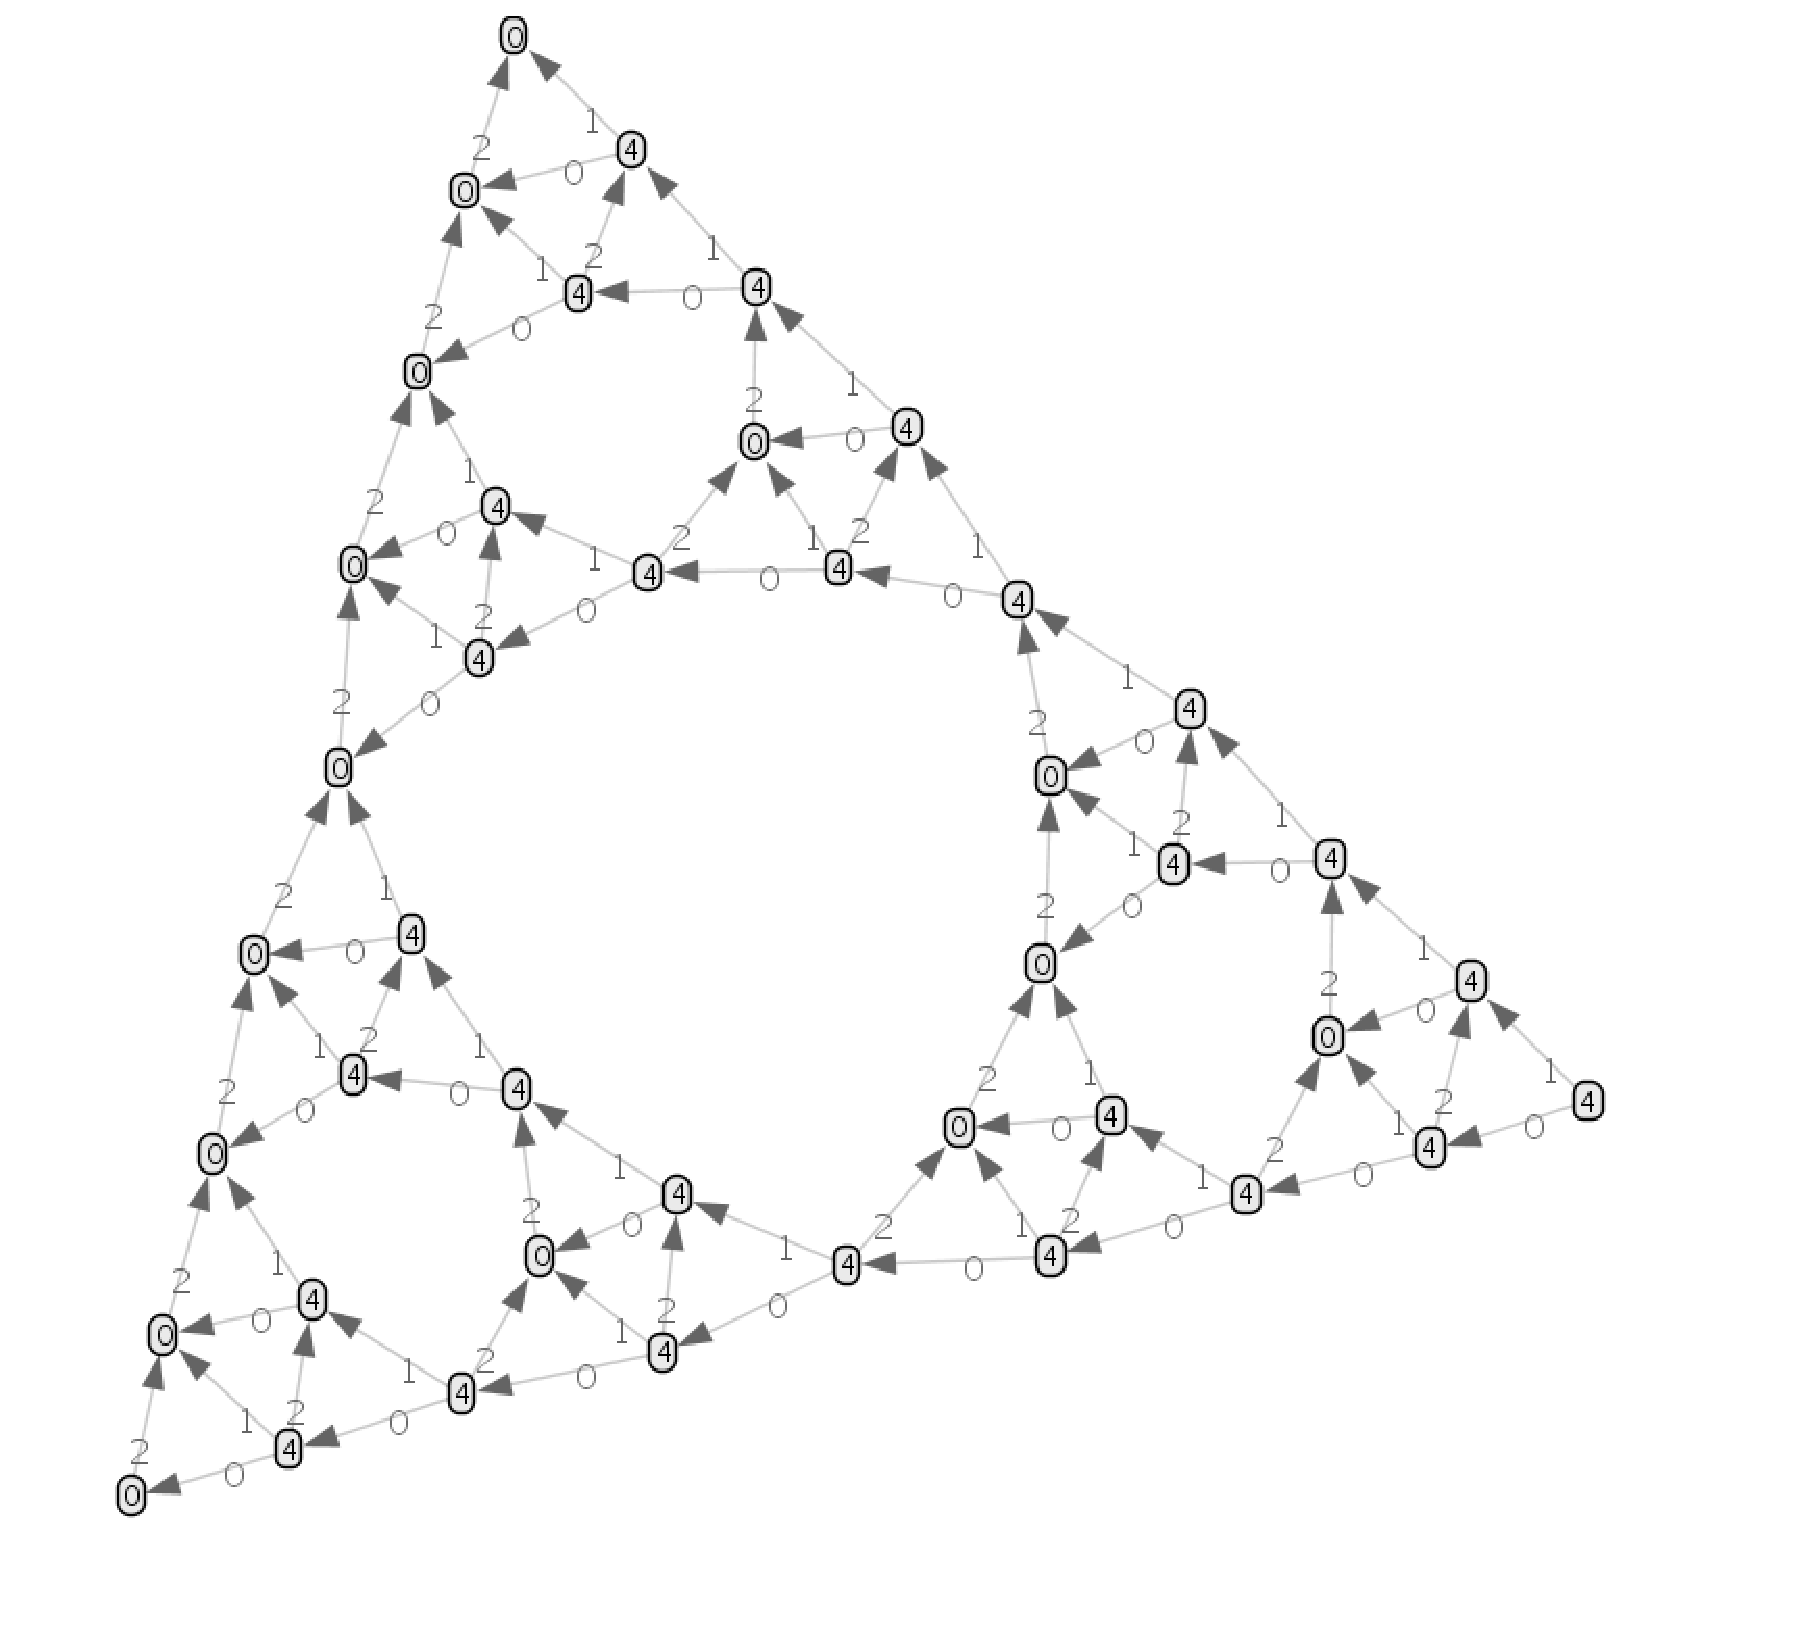
\includegraphics[scale=.4,angle=-15]{sierpinski-3.eps}
 \end{center}
\vspace*{-2.5cm}
\caption{Third generation Sierpinski triangle \label{fig:sierpinski}}
\end{figure}




\section{Implementation}

An flowchart of the reference interpreter is shown in Figure \ref{fig:architecture}. Following that, we present a detailed look at each individual component.

\subsection{Overview}

\begin{figure}
\centering
\begin{tikzpicture} [align=center, arrowout]

\node(parser) at (0,0)  [box, rounded corners] {Parser};

\node(gen) at (3,0) [box, rounded corners] {Transformer};

\node(inter) at (6.5,0) [box, rounded corners] {Interpreter};

\node(apply) at (4.5,-2) [box, rounded corners] {Rule Applier};

\draw[arrowout] (-2, 0.22) -- node[above, text width=1.5cm]{\scriptsize{Host Graph File}} (parser.160);
\draw[arrowout] (-2, -0.22) -- node[below, text width=1.5cm]{\scriptsize{Program File}} (parser.200);
\draw[arrowout] (0,-1.7) -- node[right, text width=1.5cm]{\scriptsize{Rule Application Bound}} (parser.270);

\draw [arrowout] (parser) --  (gen);
\node at (1.35,0.3) {\scriptsize{AST}};

\draw [arrowout] (gen.10) -- node[above, text width=1cm]{\scriptsize{Host Graph}} (inter.167);
\draw [arrowout] (gen.350) --  (inter.193);
\node at (4.9,-0.5) [text width=1cm]{\scriptsize{Program}};

\draw [arrowout] (inter.325) |- (apply.350);
\node at (7.8,-1.3) {\scriptsize{Rule}};

\draw [arrowout] (inter.310) |- (apply.10);
\node at (6.4, -1.3) [text width=1cm]{\scriptsize{Host Graph}};

\draw [arrowout] (apply.90) --  (inter.225);
\node at (4.6,-1) {\scriptsize{Graphs}};

\draw[arrowout] (inter) -- node[above, text width=1cm]{\scriptsize{Output Data}} (8.5,0);

\end{tikzpicture}



\caption{Data flow of the reference interpreter.} \label{fig:architecture}
\end{figure}

The interpreter takes three inputs: a file containing the textual representation of a GP2 program, a file containing the textual representation of a host graph, and an upper limit on the number of rule applications to be made before halting program execution. The interpreter runs the program on the host graph until either the bound is reached or the end of the program is reached on all branches. The default output is a complete description of all possible outputs. There is a command-line flag to print only one result in case the total computation is too slow for a particular program.

\subsection{Parser}

We use a parser combinator library fine-tuned to process some syntax specific to GP2. Each nonterminal of the GP2 context-free grammar is a function that parses the right-hand side of its rule. These functions are chained together with combinators. The combinators facilitate the requirements of the parsing step. For example, there is a combinator to parse zero or more of a string, and a combinator to ignore a token with no semantic significance. 

\subsection{Transformation}

The transformation phase extracts some semantic information from the AST, such as the types of variables specified in a rule schema's parameter list, and transforms graphs into an internal representation.

A graph is represented as a pair of extensible arrays: one for the nodes and one for the edges. An array is a list of key-value pairs, where the keys are integers. Node and edge labels are encoded into the node and edge data types. The simplicity of this implementation is intentional. Operations on graphs are concisely represented using Haskell's library of list processing functions. We chose to emphasise simplicity, readability and elegance over performance.

\subsection{The Interpreter}

The interpreter runs the GP2 program on the host graph. In many example programs, the same graph can be reached through several distinct computational branches. Therefore, when program execution is complete, a naive isomorphism checker is used to collate the list of output graphs into its isomorphism classes. The output is as follows:

\begin{itemize}
\item A list of unique output graphs, up to isomorphism, with a count of how many isomorphic copies of each graph were generated.
\item The number of failures. A failure occurs when no rule from a set of rules cannot be applied to a graph, except if the rule set is in a loop or the conditional section of a conditional branching statement.
\item The number of unfinished computations. A computation is unfinished if the bound on rule applications has been reached before the end of the program.
\end{itemize}

During program execution, a list of \texttt{GraphStates} is maintained, representing every possible nondeterministic execution of the program. A \texttt{GraphState} is an abstract data type: its values are a graph along with its rule application count, a failure symbol, and an unfinished symbol. There is a Haskell function to evaluate each GP2 control construct. Each function takes as input a single \texttt{GraphState}, along with some data about the program, and outputs a list of \texttt{GraphStates}. The \texttt{GraphStates} are propagated between functions with the use of recursive calls and Haskell's \texttt{concatMap} function. \texttt{GraphStates} representing failures and unfinished computations remain untouched after their creation, while \texttt{GraphStates} containing an intermediate graph are modified when a rule call is reached in the program's AST. The rule application process is the core of the interpreter, which is discussed in the following sections.


\subsection{Graph Matching}

From a pattern graph $L$ and a host graph $G$, the graph matcher constructs a list of \texttt{GraphMorphisms}. A \texttt{GraphMorphism} is a data structure containing the \textit{environment}, namely the variable-value assignments; a mapping between nodes in $L$ and the corresponding nodes in $G$; and a similar list of edge mappings. Morphisms are generated in two steps. First the node morphisms are constructed, then each node morphism is augmented with appropriate edge mappings if possible. The mappings used are association lists. Like our graph representation, they are simple and easy to manage at the expense of performance.

The node matching algorithm works as follows, where $k$ is the number of nodes in $L$. 

\begin{enumerate}
\item Generate the list of all $k$-sized sets of nodes from $G$.
\item Pair up (with Haskell's \texttt{zip}) each of the above sets with the set of nodes from $L$ to create a list of candidate node morphisms.
\item Remove items from the candidate morphisms list that:
  \begin{itemize}
  \item map a root node to a non-root node.
  \item map a node $l$ to a node $h$ where either the indegree or outdegree of $l$ is greater than that of $h$.
  \item map a node $l$ to a node $h$ where $l$'s mark is not cyan and not equal to $h$'s mark.
  \end{itemize}
\item Iterate through the sets from step 2, comparing the labels of nodes in $L$ to those in $G$. Remove the sets in which node labels do not match for all pairs of nodes. Add any variable-value assignments as necessary.
\end{enumerate}

The three filtering criteria in step 3 are cheap relative to label matching because they perform comparisons on easily-accessible information, in contrast to a full scan of a potentially large GP2 list expression.

It is clear that the complexity of this algorithm increases exponentially with both the size of $L$ and the size of $G$ due to the expensive first step. This is a naive matching strategy that would not be appropriate if performance were a consideration. In this case, where correctness is a greater concern, the simplicity of this algorithm is of benefit by making the source code easier to reason about.


The edge matching algorithm attempts to find an appropriate edge morphism for each node morphism in the list generated above. Valid edge morphisms are added to the data structure and returned as a \texttt{GraphMorphism}. The first step is to generate the list of source-target pairs of each edge in $L$. Then, for each node morphism $NM$:

\begin{enumerate}
\item Translate each source and target pair from $L$ to the pair of their images in $G$, according to $NM$.
\item For each source-target pair in $G$, get the list of edges from the source to the target.
\item Using a zip operation, pair each edge in $L$ with its set of candidate edge matches from the previous step.
\item For each edge in $L$, test its label against the labels of all of its candidate matches. Remove the items in which edge labels do not match. Add any variable-value assignments as necessary.
\end{enumerate}

In this way, the morphisms generated obey the morphism conditions by construction. Furthermore, all morphisms generated are total morphisms. This is because the collection of \textit{all} nodes (edges) in $L$ were tested against candidate node (edge) sets of equal size.


\subsection{Label Matching}

The label matching algorithm establishes whether a label from a rule item can be matched with a label from a host item. It takes as input the current environment and the two labels to be compared. 

GP2 labels consist of a mark and a list. The marks are encoded as an abstract data type and are directly comparable. Lists are naturally represented as Haskell lists, where each element is an atom. Atoms occurring in the host graph are constants (integers, characters or strings), while rule atoms are either constants, variables or a concatenated string. If a variable-value assignment is required to a complete a match, it is tested against the current environment to ensure that the same variable is not mapped to two different values. 

In almost all cases, atoms are directly comparable. The most interesting case occurs if a list variable is encountered. We exploit the fact that only one list variable is allowed in a LHS label (to ensure unique matches). The length of the remainder of the rule list is compared with the length of the remainder of the host list. This information is used either to assign the list variable the list of appropriate length, or to abort matching in the case that there are too few host atoms left to match the remaining rule atoms.

\subsection{Rule Application}

If the graph matcher returned a list of morphisms, each of these morphisms is checked against the dangling condition and any application conditions in the rule itself. Following that, the rule application is performed in the following steps: delete edges, delete nodes, relabel nodes, add nodes, relabel edges, add edges. 

The output of the rule application is a list of graphs, where each graph is the result of a single rule application guided by one of the morphisms returned by the graph matcher.

%In the double-pushout framework of graph transformation, on which GP 2 is based, a rule may not be applicable for a particular match as applying the rule could leave an edge without a source or target. The dangling condition forbids this: it requires that all host edges not deleted by the rule are not incident to nodes deleted by the role.


%\subsection{Rooted graphs}

%Lessons learned from the implementation of the original GP language led to the addition of support for root nodes to GP2. A node carries a simple binary flag indicating whether it is a root node or not. A root node in a rule graph can only match a root node in the host graph, and then only if all other normal matching conditions are met, eliminating a large number of possible subgraph matches with only an inexpensive boolean test. Whereas a non-root node in the rule graph may match a node irrespective of its root-node status.


%Even in the reference interpreter, addition of a root node can result in a significant performance gain.

